\documentclass{beamer}
%\usepackage[T1]{fontenc}
%\usepackage{cmbright}
\usepackage{graphicx}
\usepackage{subcaption}
\usepackage{epstopdf}
%\usepackage{subfig}
%\usepackage{subfigure}
\usepackage{booktabs}
%\usepackage[english]{babel}
%\usepackage{setspace}
%\usepackage{multirow}
\usepackage{amsmath}
\usetheme{boxes}

\setbeamercolor{mycolor}{fg=red}

\AtBeginSection[]{
  \begin{frame}
  \vfill
  \centering
  \begin{beamercolorbox}[sep=8pt,center,shadow=true,rounded=true]{mycolor}
    \usebeamerfont{title}\insertsectionhead\par%
  \end{beamercolorbox}
  \vfill
  \end{frame}
}

\mode<presentation>
{
    \setbeamercovered{invisible}
}
%\usetheme{Boadilla}
%\usecolortheme{seahorse}
%\usecolortheme{rose}
%\setbeamercovered{transparent}

\title [Dynamic Perturbation] {Dynamic Perturbation}

\author[Mennuni and Stepanchuk]{Alessandro Mennuni and Serhiy Stepanchuk \\ (University of Southampton)}

\date[June 19, 2018]{June 19, 2018 \\ CEF2018}

\begin{document}

\begin{frame}
\titlepage
\end{frame}

\section{Introduction}

\begin{frame}{Motivation}

    2 main methods of solving dynamic models:

    \medskip
    \begin{enumerate}
        \item Local perturbations:
            \begin{itemize}
                \item accurate solution around the point of approximation -- normally a steady state
                \item fast, can handle many state variables
                \item quality of solution may deteriorate far from approximation point or 
                    with large nonlinearities
            \end{itemize}
        \item Global projection methods:
            \begin{itemize}
                \item accurate solution on the whole (or large part of) state space
                \item costly, suffers from the ``curse of dimensionality''
            \end{itemize}
    \end{enumerate}

    \bigskip
    In many applications, we want accurate solution along a single simulated path.

\end{frame}

\begin{frame}{What we do}

    \begin{enumerate}
        \item We develop a hybrid solution method:

            \begin{itemize}
                \item constructs a sequence of local approximations along the simulated path
                \item provides accurate approximation exactly where we need it
                \item can handle models with large number of state variables
                    and/or nonlinearities (e.g. borrowing constraints)
            \end{itemize}
        \item Test our solution in multi-country ... model, compare 
            it to Maliar and Maliar
        \item Test our solution in a model of sudden stops
        \item The basis for estimation based on Kalman filter with
            time-varying coefficients
    \end{enumerate}
        
\end{frame}

\begin{frame}{Related Literature}

\begin{itemize}
    \item PEA and Maliar/Maliar
    \item Den Haan
    \item New Maliars paper?
    \item Fair/Taylor? 
\end{itemize}

\end{frame}

\section{Algorithm}

\begin{frame}{Setup and notation}
    \begin{itemize}
        \item Equilibrium is described by the \emph{equilibrium sytem of equations}:
            \[
                E_t \left[ f(x_t,y_t,x_{t+1},y_{t+1}) \right]  = 0
            \]
            where $x_t$ is a vector of state variables, $y_t$ is the vector 
            of control (jump) variables.

        \item We look for recursive solution in the form of the policy functions
            for the control variables:
            \[
                y_t = g(x_t,\sigma)
            \]
            and next-period states:
            \[
                x_{t+1} = h(x_t,\sigma) + \sigma \eta_{t+1}
            \]
            where $\eta_t$ are \emph{innovations}, $\sigma$ controls their magnitude.

        \item In the current version, we limit ourselves to the first-order
    approximations where certainty equivalence holds.
    \end{itemize}

\end{frame}

\begin{frame}{Idea}

    \begin{itemize}
        \item We want to find a dynamic sequence solution 
            $\{x^{seq}_0, x^{seq}_1, \ldots \}$ for
            a given $x^{seq}_0$ and innovations $\{ \eta_1, \eta_2, \ldots \}$
            \bigskip
        \item Stardard perturbation solution: use Taylor approximation
            of the equilibrium system around the steady state:
            \[
                f(\bar{x}, \bar{x}, \bar{y}, \bar{y}) = 0
            \]
            \medskip
        \item Can be of poor quality far from $\bar{x}$ or in highly
            nonlinear model. Can we do better?
            \bigskip
        \item One can use Taylor approximation around any other point
    $(x_t,x_{t+1},y_t,y_{t+1})$ that solves the equilibrium 
    system.
            \bigskip
        \item How do we find such a point for arbitrary $x_t = x_0$?
    \end{itemize}

\end{frame}

\begin{frame}{Finding local dynamic point solution}
    Starting with $x_0=x^{seq}_0$, we trace 2 auxilliary paths:
    \begin{enumerate}
        \item \emph{Forward path:}
            \begin{itemize}
                \item using steady state policy functions
                \item construct $\{x_0,x^{fp}_1,\ldots,x^{fp}_T\}$ with 
                    $x^{fp}_T$ close to $\bar{x}$
            \end{itemize}
        \item \emph{Backward path:}
            \begin{itemize}
                \item[(a)] trace the ``forward path'' backwards towards $x_0$
                \item[(b)] start with $x^{fp}_T$ and assume that next-period
                    control variables can be computed using steady-state
                    policy function, $y_{T+1} = g_{\bar{x}}(x_{T+1})$
                \item[(c)] solve the equilibrium system for $x_{T+1}$ and $y_T$:
                    \[
                        f(x^{fp}_T, y_T, x_{T+1}, g_{\bar{x}}(x_{T+1})) = 0
                    \]
                \item[(d)] Taylor approximate the equilibrium system
                    around this solution point, get a new policy function
                    $g = g_{x^{fp}_T}$
                \item[(e)] move to the previous point in the forward path, $x^{fp}_{T-1}$, set $g = g_{x^{fp}_T}$, and repeat steps (c) and (d)
                \item[(f)] keep moving backwards until $x_0$ is reached
                        
            \end{itemize}
    \end{enumerate}
\end{frame}

\begin{frame}{Updating dynamic sequence solution}
    When we reach the last step in the \emph{backward path},
    we have both 
    \begin{itemize}
        \item a point solution to:
            \[
                f(x^{seq}_t,y_t,x_{t+1},y_{t+1}) = 0
            \]
        \item approximation to policy functions $h_{x^{seq}_t}$ and $g_{x^{seq}_t}$
    \end{itemize}

    \bigskip
    We combine these policy functions and the realization of the innovations $\eta_{t+1}$ to compute the next elements in our \emph{dynamic sequence solution}:
    \[
        x^{seq}_{t+1} = h_{x^{seq}_t}(x^{seq}_t) + \sigma \eta_{t+1}
    \]

    \bigskip
    Next, we trace the \emph{forward} and \emph{backward} paths starting 
    with $x_0 = x^{seq}_{t+1}$.
\end{frame}

\section{Multi-country RBC model}
\begin{frame}{Setup}
    \begin{itemize}
        \item N countries 
        \item Country-specific productivity shocks
        \item Planner solves:
            \small
            \begin{align*}
                \max & \; E_0 \sum_{i=1}^N \lambda^i \sum_{t=0}^{\infty} \beta^t \log(c^i_{t}) \\
                \text{s.t.:} & \\
                             & \sum_{i=1}^N c^i_{t} + \sum_{i=1}^N k^i_{t+1} = \sum_{i=1}^N k^i_{t}(1-\delta) + \sum_{i=1}^N a^i_{t} f(k^i_{t}), \\
                             & \ln a^i_{t+1} = \rho \ln a^i_t + \varepsilon^i_{t+1}, \; \varepsilon^i \sim \mathbf{N}(0,\sigma_i) \\
                             & \{k^i_0,a^i_0\}_{i=1}^N \quad \text{are given}.
            \end{align*}
            \normalsize
    \end{itemize}
    We compare our solution to ``$\varepsilon$-distinguishable set'' (EDS) algorithm 
    from Maliar \& Maliar (2015):
    \begin{itemize}
        \item a cutting-edge global solution approach to high dimensional problems
    \end{itemize}
    
\end{frame}

\begin{frame}{Euler equation errors in 2-country case}

    \begin{figure}[htpb]
        \centering
        %\caption{Euler equation errors}
        \label{fig-eulererrors_2countries_baseline}
        \begin{subfigure}[b]{0.50\textwidth}
            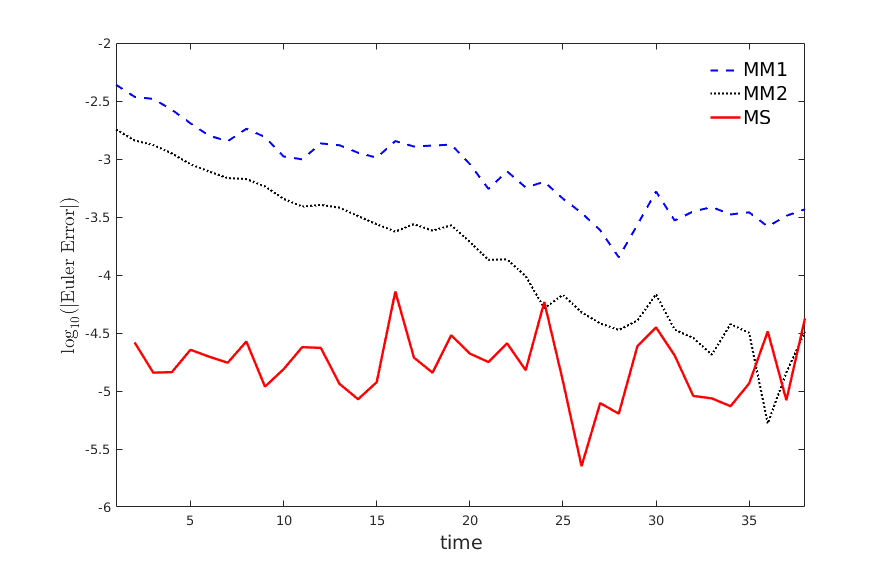
\includegraphics[width=\textwidth]{two_country_0_1_k0_0_5_euler_errors}
            \caption{$k_0=0.5 k_{ss}$}
            \label{two_country_k_0_low}
        \end{subfigure}
        \begin{subfigure}[b]{0.48\textwidth}
            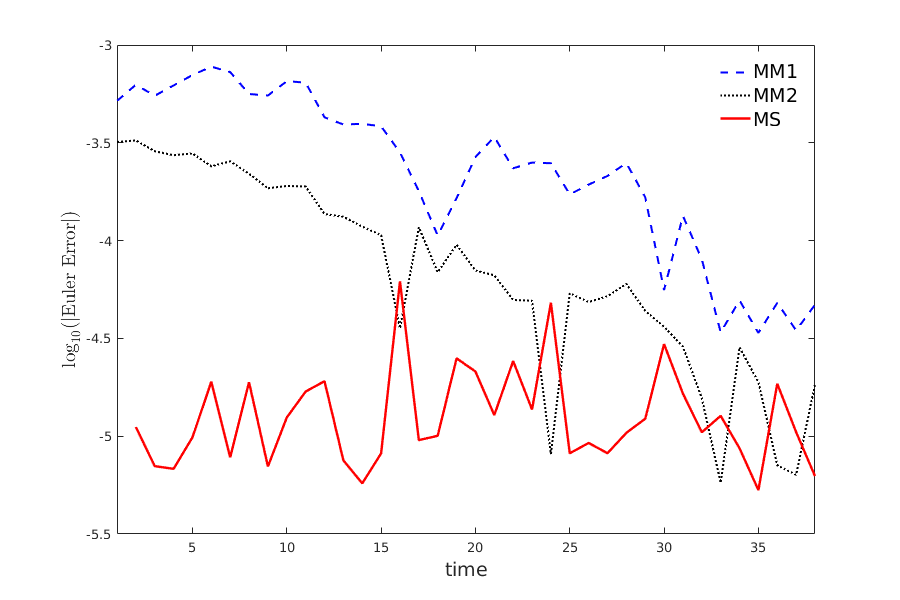
\includegraphics[width=\textwidth]{two_country_0_1_k0_1_5_euler_errors}
            \caption{$k_0=1.5 k_{ss}$}
            \label{two_country_k_0_high}
        \end{subfigure}
    \end{figure}

    \small
    We compare our results (MS) to Maliar \& Maliar's EDF with first- (MM1) and second-order (MM2)
    polynomials.

    \medskip
    We set $\sigma_i = 0.01$ and same $k_0$ in both countries.
    
\end{frame}

\begin{frame}{Changing shock volatility}
    \begin{figure}[htpb]
        \centering
        %\caption{Euler equation errors, changing the volatility of shocks}
        \label{fig-eulererrors_2countries_changingsigma}
        \begin{subfigure}[b]{0.49\textwidth}
            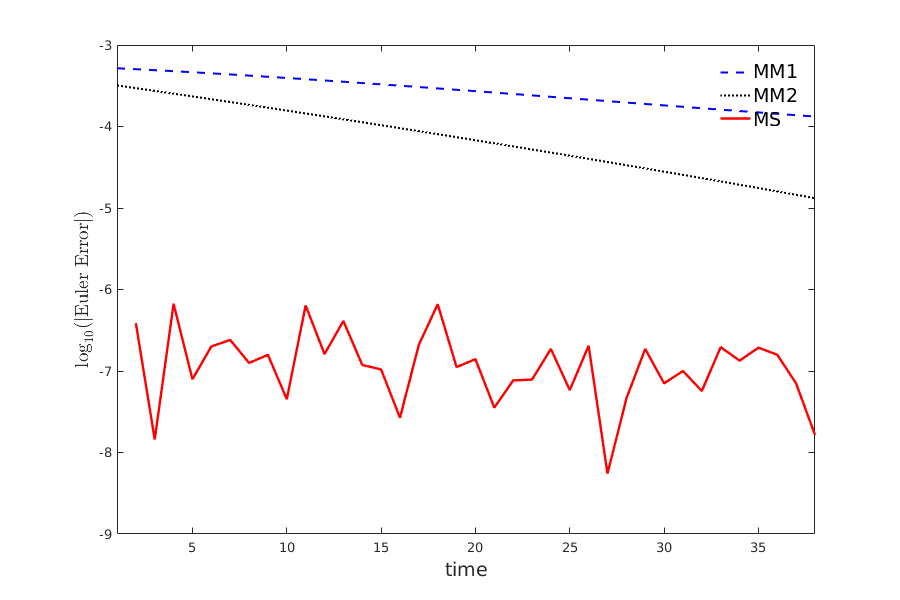
\includegraphics[width=\textwidth]{two_country_sigmasmall_k0_1_5_euler_errors}
            \caption{$\sigma=10^{-6}$}
            \label{two_country_sigma_low}
        \end{subfigure}
        \begin{subfigure}[b]{0.49\textwidth}
            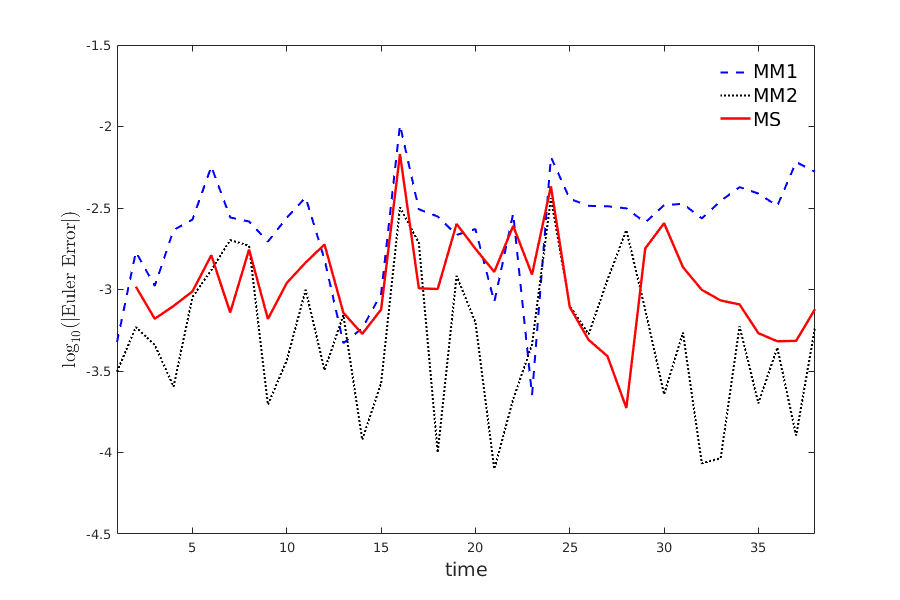
\includegraphics[width=\textwidth]{two_country_sigmalarge_k0_1_5_euler_errors}
            \caption{$\sigma=0.1$}
            \label{two_country_sigma_high}
        \end{subfigure}
    \end{figure} 

    \small
    Our method is based on local first-order approximations, which imply certainty equivalence.

    \medskip
    This becomes more important with larger shocks.
    
\end{frame}

\begin{frame}{Accuracy and speed with large N}
    %\begin{table}
        %\label{tab:n_countries_summary}
        %\scalebox{0.8}{
            %\centering
            %\begin{tabular}{cccccccccc}
                %\hline
                %& \multicolumn{3}{c}{N=20}  &
                %\multicolumn{3}{c}{N=40}  & \multicolumn{3}{c}{N=200}   \\
                %\cmidrule(lr){2-4} \cmidrule(lr){5-7} \cmidrule(lr){8-10}
                 %& $L_1$ & $L_{\infty}$ & CPU &
                %$L_1$ & $L_{\infty}$ & CPU
                      %& $L_1$ & $L_{\infty}$ & CPU \\
                %\hline
                %MM1 & -4.27 & -3.01 & 188.18 &-4.28 & -2.98 & 244.70 & -4.29 & -2.94 & 792.27 \\
                %MM2 & -4.85 & -3.41 & 1399.21 & -4.94 & -3.48 & 12105.21 & \\
                %MS  & -5.43 & -4.43 & 24.31 & -5.42 & -4.53 &
                %58.01 & -5.42 & -4.70 & 390.92 \\
            %\end{tabular}
        %}
    %\end{table}

    \begin{table}
        \label{tab:n_countries_summary}
        \scalebox{0.8}{
            \centering
            \begin{tabular}{ccccccc}
                \hline
                &
                \multicolumn{3}{c}{N=40}  & \multicolumn{3}{c}{N=200}   \\
                \cmidrule(lr){2-4} \cmidrule(lr){5-7} 
                Soln Method & $L_1$ & $L_{\infty}$ & CPU &
                $L_1$ & $L_{\infty}$ & CPU \\
                \hline
                MM1 &-4.28 & -2.98 & 244.70 & -4.29 & -2.94 & 792.27 \\
                MM2 & -4.94 & -3.48 & 12105.21 & \\
                MS  & -5.42 & -4.53 &
                58.01 & -5.42 & -4.70 & 390.92 \\
                \hline
            \end{tabular}
        }
    \end{table}

    \bigskip
    \small
    For large $N$ ($N \geq 40$), one-node Gauss-Hermite integration appears 
    to be the only viable option for EDF.
\end{frame}

\section{Sudden stops model}


\begin{frame}{Setup}
    \small
    \begin{itemize}
        \item Model from Mendoza (2010) 
        \item Small open economy with a representative consumer/firm owner who maximizes:
            \footnotesize
            \begin{align*}
                \max & E_0 \left( \sum_{t=0}^{\infty} \exp \left( - \sum_{\tau=0}^{t} \rho \left(
                            \bar{c}_{\tau} -
                N(\bar{L}_{\tau}) \right) \right) u\left(c_t - N(L_t)\right) \right) \\
                \text{s.t.:} & \\ 
                (1+\tau_c) & c_t + i_t + q_t^b b_{t+1} = \exp(\varepsilon^A_t) F(k_t, L_t) - \phi(R_t-1) w_t L_t + b_t, \\
                i_t & = \delta k_t + (k_{t+1} - k_t) \left(1 + \Psi\left(\frac{k_{t+1}-k_t}{k_t}\right) \right)
            \end{align*}
        \item Additionally, there is (occasionally binding) collateral borrowing constraint:
            \[
                q^b_t b_{t+1} - \phi R_t w_t L_t \geq -\kappa q_t k_{t+1}
            \]
        \item $\varepsilon^A$ is TFP shock, $R_t = R \exp(\varepsilon^R_t)$ where $\varepsilon^R$ is interest rate shock.
        \item $\rho(.)$ is an increasing and concave ``endogenous discount factor'' that ensures unique steady state
    \end{itemize}
    
\end{frame}

\begin{frame}{Occasionally binding constraint}
    To incorporate occasionally binding constraint in equilibrium system of equations, we 
    use a utility penalty function:
    \[
        K \cdot \max\left( -(\kappa q_t k_{t+1} + q^b_t b_{t+1} - \phi R_t w_t L_t)^d , 0\right)
    \]
    with large $K > 0$ and $d \in \{2,4\}$.

    It is ``activated'' only when the constraint is violated.

    \bigskip
    \bigskip
    \bigskip
    Alternatively, one can use Garcia-Zangwill trick.
\end{frame}

\begin{frame}{Simulated path}

    \begin{figure}[htpb]
        \centering
        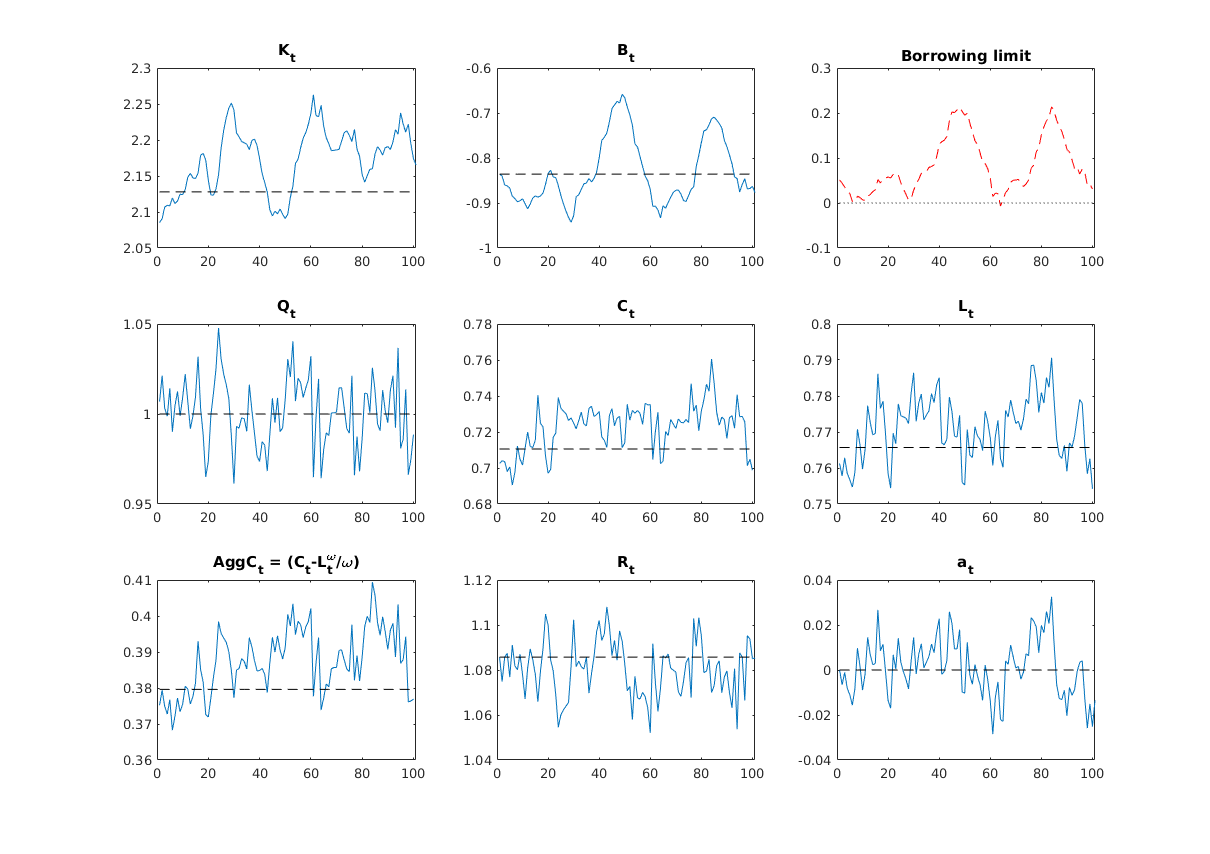
\includegraphics[width=1.0\linewidth]{sudden_stops_path}
        %\caption{sudden_stops_path}
        \label{fig:sudden_stops_path}
    \end{figure}
    
\end{frame}

\section{Kalman Filter}

\begin{frame}{Idea}
    \begin{itemize}
        \item Our algorithm produces an accurate solution for a single simulated path
            \bigskip
        \item Ideal for estimation based on a given sequence of observations
            \bigskip
        \item We get a sequence of policy functions along the simulated path
            \bigskip
        \item So, we can use Kalman filter with varying coefficients
            \bigskip
        \item We use the ``sudden stops'' model as our test lab
    \end{itemize}
\end{frame}

\begin{frame}{Extended Kalman Filter}
    
\end{frame}

\begin{frame}{Iterated Extended Kalman Filter}
    
\end{frame}

\begin{frame}{State-space formulation}
    State vector:
    \begin{itemize}
        
    \end{itemize}
    
    \bigskip
    Observations:
\end{frame}


\end{document}


